\chapter{Zastosowania}
\label{cha:zastosowania}

\section{Choroby serca i pierwsza pomoc przy zawale}

Obecne społeczeństwo najwięcej kłopotów zdrowotnych ma z układem krążenia. Choroby serca są najbardziej rozpowszechnione na świecie, zwłaszcza w krajach wysoko rozwiniętych. Dlatego niezmiernie ważne jest nie tylko leczenie, ale także i zapobieganie chorobom i rehabilitacja po zawale.
\subsection{Telefony komórkowe a pierwsza pomoc}

W przypadku zawału serca niezbędna jest szybka reakcja. Często jednak stres uniemożliwia poprawne udzielenie pierwszej pomocy. Z pomocą przychodzą nam coraz szerzej dostępne inteligentne telefony komórkowe - smartphone'y. W czasopiśmie "Interventional Cardiology" (\cite{ICHoneyman2014Mobilehealthapplicationsincardiaccare}) opisane jest, w jaki sposób aplikacja mobilna może pomóc w przeprowadzeniu akcji rehabilitacyjnej:
\begin{figure}[ht!]
  \centering
    \reflectbox{%
      \includegraphics[width=0.5\textwidth]{images/cpr}}
  \caption{Schemat akcji resuscytacyjnej przy pomocy smartphone'a}
\end{figure}

\subsection{Pomoc po zawale}

Po zawale serca bardzo ważna jest praca nad stanem układu krążenia. Często jednak odległość do najbliższego szpitala jest czynnikiem zaporowym, uniemożliwiającym poprawne zadbanie o zdrowie. Ostatnie badania pokazują jednak \cite{FMottl2014Smartphoneappprovesvaluableforcardiacpatients}, iż telefon komórkowy może znacznie poprawić sytuację pacjentów pozawałowych. Aplikacja przypomina o regularnych ćwiczeniach i pozwala monitorować aktualny stan zdrowia.
\section{Monitorowanie pacjenta chorego na cukrzycę}
\label{sec:cukrzyca}

Problem cukrzycy jest również jednym z najpoważniejszych zadań, z jakimi spotyka się dzisiejsza medycyna. Dotyczy on bowiem znacznej części społeczeństwa. W artykule \cite{CDTran2012Smartphone-BasedGlucoseMonitorsandApplicationsintheManagementofDiabetes:AnOverviewof10SalientAppsandaNovelSmartphone-ConnectedBloodGlucoseMonitorUnitedStates--USGlucoseSmartphonesCellulartelephonesDiabetes} możemy znaleźć informacje na temat dostępnych na rynku aplikacji do monitorowania poziomu cukru we krwi.
\subsection{Przegląd aplikacji}
Na rynku dostępnych jest wiele aplikacji na wszystkie popularne obecnie platformy, takie jak Android, iOS czy BlackBerry OS.
\paragraph{Glucose Buddy}\mbox{}\\
Aplikacja firmy SkyHealth integruje funkcjonalność smartphone'a z danymi dostępnymi w internecie. Użytkownik może śledzić nie tylko swój poziom cukru we krwi, ale także na przykład ilość przyjmowanych składników spożywczych. Aplikacja jest darmowa.
\paragraph{Diabetes Buddy}\mbox{}\\
Płatną, ale bardziej rozwiniętą aplikacją, jest Diabetes Buddy. Umożliwia ona także monitorowanie poziomu ciśnienia krwi.
\paragraph{Log Frog}\mbox{}\\
Jedną z ciekawszych propozycji na rynku jest aplikacja Log Frog. Oferuje ona opisane wcześniej funkcjonalności, różni się jednak bardzo przyjaznym i prostym interfejsem, odpowiednim dla dzieci bądź osób starszych.

\section{Aplikacja mobilna a choroby psychiczne}
Okazuje się, iż telefony komórkowe obecnie mogą pomóc nie tylko osobom chorym z powodu dysfunkcji narządów. Także pacjenci mentalnie chorzy mogą liczyć na pomoc dzisiejszej technologii. Za pomocą odpowiednich systemów monitorowane są ich zachowania w konkretnych sytuacjach, przez co osobom opiekującym się nimi łatwiej jest dostrzec nieprawidłowości.\\
Do tej pory prowadzone badania obejmowały m. in. schizofrenię i psychozę oraz chorobę dwubiegunową \cite{IJOMHSPawelProciow2012Mobilepsychiatry:towardsimprovingthecareforbipolardisorderScience&TechnologyLifeSciences&BiomedicinePsychiatryPSYCHIATRYSSCIAMBULATORYASSESSMENTCIRCADIAN-RHYTHMSMENTAL-DISORDERSDAILY-LIFEPSYCHOLOGYCREATIVITYMOVEMENTBURDENSLEEP}. W artykule \cite{JoPNHSElias2014MobileAppsforPsychiatricNursesPsychiatric-mentalhealthnursingSmartphonesHandheldcomputersSoftware} omówione zostały aplikacje przydatne specjalistom w dziedzinie psychologii. \\ \\ \\
\begin{figure}[ht!]
  \centering
    \reflectbox{%
      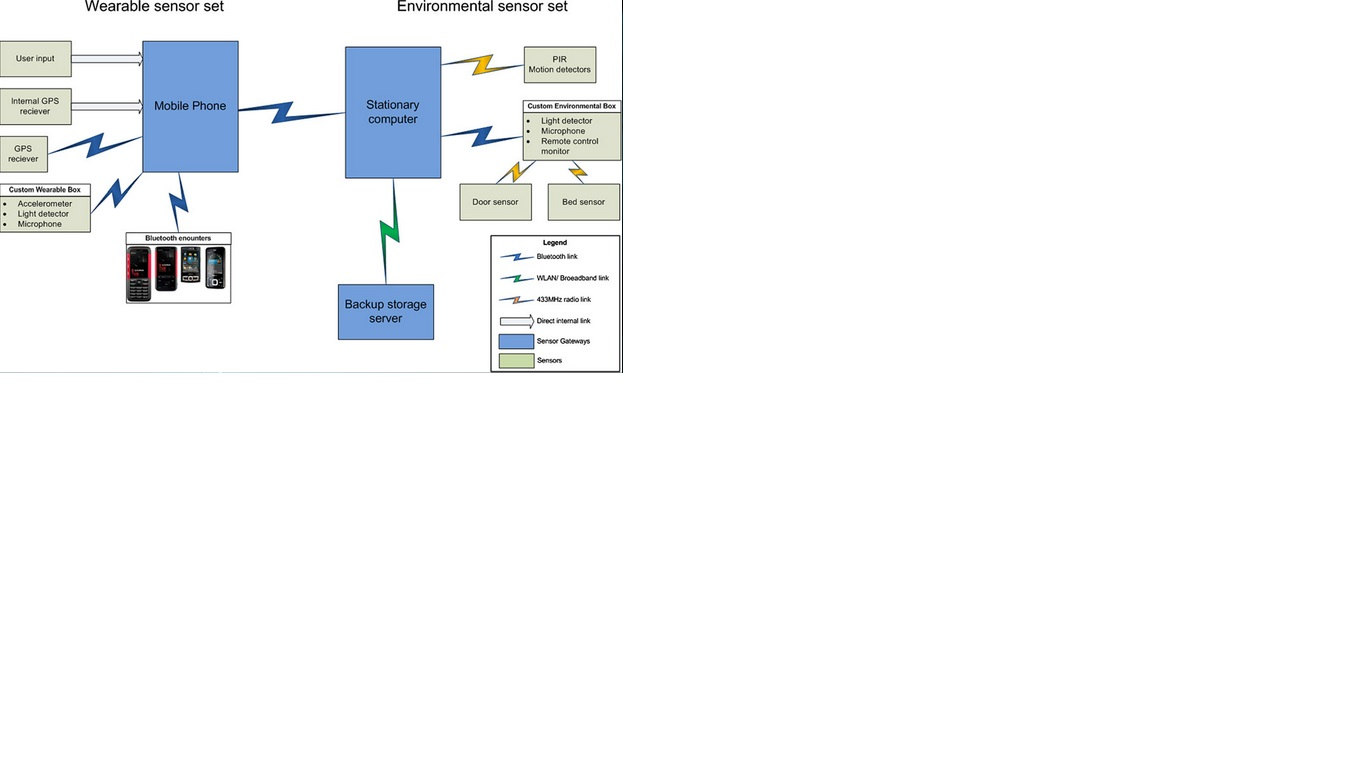
\includegraphics[width=0.5\textwidth]{images/psychic}}
  \caption{Schemat aplikacji badającej zachowania pacjenta chorego psychicznie}
\end{figure}
\section{Akcelerometr  w leczeniu choroby parkinsona}
Również choroby neurodegeneracyjne mają swoją szufladę w dziedzinie rozwoju technologii mHealth. Badania pokazują (\cite{AICPSSanders2013RemotesmartphonemonitoringformanagementofParkinsonsDiseaseEEGaccelerationactivitymonitoringelectroencephalogrammobilecomputingsensorsmart-phonewatchwrist}), iż regularne monitorowanie stanu zdrowia pacjenta może znacznie opóźnić rozwój choroby. Niestety częste wizyty w szpitalu dla wielu pacjentów są nieomal nieosiągalne. Dlatego też podręczne urządzenia, takie jak smartphone'y, okazują się tu nieocenione. Jeden z największych koncernów - Intel \cite{BMacKellar2014AussiemhealthfirmtorollouttoolforParkinsons} - pracuje nad technologią przenośnych "gadżetów", które chory mógłby nosić w celu monitorowania stanu zdrowia.
\section{Leczenie i kontrolowanie uzależnień}
Kolejnym z problemów, z jakim spotyka się obecna medycyna, jest uzależnienie od leków. Nadużywanie przepisanych medykamentów, co dotyczy zwłaszcza opioidów, nie tylko podwyższa koszty leczenia, ale także może prowadzić do poważnych zaburzeń zdrowotnych. W rezultacie pacjent zamiast się leczyć, pogarsza tylko swoją sytuację. Aby temu zapobiec, można skorzystać z pomocy urządzeń mobilnych. Monitorowanie przyjmowania odpowiednich dawek leków, czy to poprzez wprowadzanie danych przez pacjenta, czy nawet dzięki urządzeniom pomiarowym, noszonym przy ciele, może pomóc wykryć pewne wzorce, wskazujące na wysokie ryzyko, iż terapia może zakończyć się uzależnieniem \cite{ISoMAHN&CVarshney2014Mobilehealth:medicationabuseandaddictionaddictionmobilehealthmonitoringprescriptionabuse}.\\
Na rysunku \ref{fig:drugs} ukazany jest przykładowy schemat takiej aplikacji.
\\ \\ \\ \\
\begin{figure}[ht!]
  \centering
    \reflectbox{%
      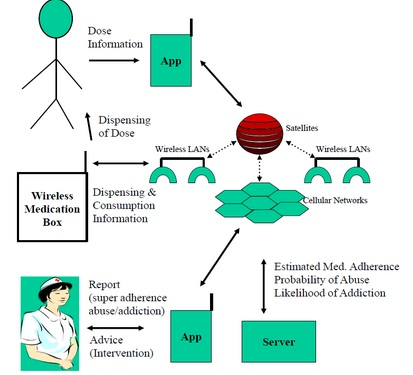
\includegraphics[width=0.5\textwidth]{images/drugs}}
  \caption{Schemat aplikacji do detekcji uzależnienia od leków}
  \label{fig:drugs}
\end{figure}

\section{Mobilna opieka nad ciążą}
W miejscach, gdzie opieka medyczna nie jest ogólnodostępna, ciąża wiąże się z ogromnym ryzykiem powikłań, które, nieleczone, często prowadzą do zgonu zarówno matki, jak i dziecka. Ponieważ technologia komórkowa w obecnych czasach jest już nieomal w stu procentach powszechna, postanowiono wykorzystać ją do pomocy przyszłym matkom, nie mogącym sobie pozwolić na częste wizyty w szpitalu. Dzięki telefonii komórkowej kobiety mogą otrzymywać nie tylko informacje o prawidłowym rozwoju ciąży i instrukcje, jak samodzielnie badać, czy dziecko rozwija się poprawnie, ale także i szybszą pomoc - istnieje specjalny system \cite{Ismaeel2013EffectiveSystemforPregnantWomenusingMobileGIS} oferujący szybką pomoc kobietom, którym grozi ryzyko poronienia, a nawet śmierci. Dzięki usługom lokalizacyjnym nawet w przypadku utraty przytomności matka ma szansę otrzymać pomoc na czas.
\begin{figure}[ht!]
  \centering
    \reflectbox{%
      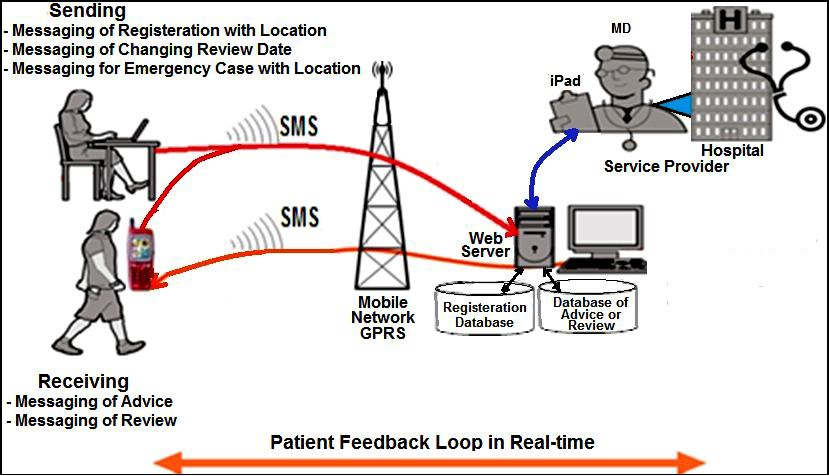
\includegraphics[width=0.5\textwidth]{images/pregnancy}}
  \caption{Budowa systemu powiadamiania i konsultacji medycznych dla kobiet w ciąży}
\end{figure}